\documentclass[11pt]{article}
\title{\textbf{Meccano polygon diagonals}}
\author{https://github.com/heptagons/meccano/penta}
\date{}

\usepackage{amsthm} % for \qed
\usepackage{../meccano}
\usepackage{longtable}

\begin{document}

\maketitle
\begin{abstract}
We construct meccano\meccanoref polygon internal diagonals.
\end{abstract}

\section{Polygon diagonals}

\begin{figure}[H]
\centering
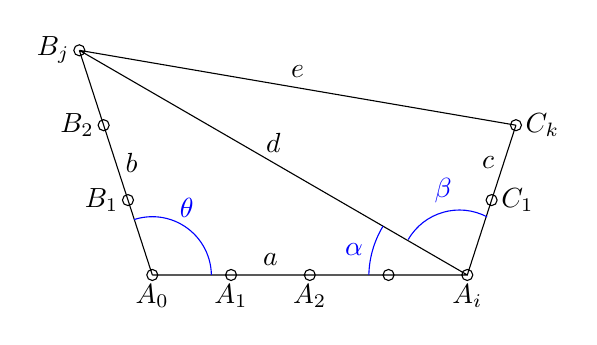
\begin{tikzpicture}
\begin{scope}[scale=1]
\begin{scope}
\draw[] (0,0) circle(2pt) node[below]{$A_i$}
-- ++(-1,0) circle(2pt)
-- ++(-1,0) circle(2pt) node[below]{$A_2$}
-- node[above]{$a$} ++(-1,0) circle(2pt) node[below]{$A_1$}
-- ++(-1,0) circle(2pt) node[below]{$A_0$}
-- ++(108:1) circle(2pt) node[left]{$B_1$}
-- node[right]{$b$} ++(108:1) circle(2pt) node[left]{$B_2$}
-- ++(108:1) circle(2pt) node[left]{$B_j$}
-- node[above]{$d$} (0,0)
-- ++(72:1) circle(2pt) node[right]{$C_1$}
-- node[left]{$c$} ++(72:1) circle(2pt) node[right]{$C_k$}
-- node[above]{$e$} ++(-5.545,0.951); % (-4-5*cos(72),sin(72))
\draw[blue] (-3.25,0) arc (0.75:108:0.75) node[midway,above]{$\theta$};
\draw[blue] (-1.25,0) arc (-1.25:-31:-1.25) node[midway,left]{$\alpha$};
\draw[blue] (-0.75,0.45) arc[start angle=90+60, end angle=62, radius=0.75] node[midway,above]{$\beta$};
\end{scope}
\end{scope}
\end{tikzpicture}
\caption{Meccano polygon three consecutive sides segments $a\ge\ b\ge c$
can form two diagonals $d$ and $e$.}
\label{fig:diagonals}
\end{figure}

\section{Regular polygon diagonals}

In the regular polygon all internal angles are equal to $\theta$.
From figure \ref{fig:diagonals} the polygon is regular if $\alpha + \beta = \theta$ so we have:
\begin{align}
\alpha &= \angle{A_0A_iB_j} \\
\beta  &= \angle{B_jA_iC_k} \\
\theta &= \angle{B_jA_0A_i} = \angle{A_0A_iC_k}\\
\alpha + \beta &= \theta
\end{align}

We use the cosines sum identity to express $\cos\beta$ in function of the rest of variables.
We define $u = \cos\theta$:
\begin{align}
u &\equiv \cos\theta\\
 &= \cos(\alpha + \beta)\\
 &= \cos\alpha\cos\beta - \sin\alpha\sin\beta\\
\sin\beta &= \frac{\cos\alpha\cos\beta - u}{\sin\alpha}\\
\sin^2\beta &= \frac{(\cos\alpha\cos\beta - u)^2}{\sin^2\alpha}\\
1 - \cos^2\beta &= \frac{\cos^2\alpha\cos^2\beta - 2u\cos\alpha\cos\beta + u^2}{sin^2\alpha}
\end{align}

We set $X = \cos\beta$ and rearrange the last equation to get:
\begin{align}
X^2 - 2u\cos\alpha X + u^2 - \sin^2\alpha &= 0
\end{align}
And solve the quadratic equation $AX^2 + BX + C = 0$ to get $\cos\beta$
in function of $u$ and $\alpha$:
\begin{align}
\cos\beta &= \frac{-B \pm \sqrt{B^2 - 4AC}}{2A}\nonumber\\
 &= \frac{2u\cos\alpha \pm 
 \sqrt{4u^2\cos^2\alpha - 4(u^2 -\sin^2\alpha)}}{2}\nonumber\\
 &= u\cos\alpha \pm \sqrt{u^2\cos^2\alpha - u^2 + \sin^2\alpha} \label{eq:cosbeta}
\end{align}

Now, we need to find the values of $\cos\alpha$, $\sin\alpha$ and $\cos\beta$ which
in turn need the value of $d$, all in terms of $a,b,c$ the segments of the polygon perimeter.
\\\\
For the value of $d$ we use the law of cosines:
\begin{align}
d &= \sqrt{a^2 + b^2 - 2ab\cos\theta} \nonumber\\
 &= \sqrt{a^2 + b^2 - 2abu} \label{eq:d}
\end{align}

Using the law of cosines we calculate the angles $\alpha =\angle{A_0A_iB_j}$ 
and $\beta =\angle{B_jA_iC_k}$:
\begin{align}
\cos\alpha &= \frac{a^2 + d^2 - b^2}{2ad} \nonumber\\
 &= \frac{a^2 + (a^2 + b^2 - 2abu) - b^2}{2ad}\nonumber \\
 &= \frac{a - bu}{d}\\
%
\cos\beta &= \frac{c^2 + d^2 - e^2}{2cd}\nonumber\\
 &= \frac{c^2 + (a^2 + b^2 - 2abu) - e^2}{2cd}\nonumber\\
 &= \frac{a^2 + b^2 + c^2 - e^2 - 2abu}{2cd}
\end{align}
We define new variable $f$ to simplify $\cos\beta$ to obtain:
\begin{align}
f &\equiv \frac{a^2 + b^2 + c^2 - e^2}{2} \label{eq:fequiv} \\
\cos\beta &= \frac{f - abu}{cd}
\end{align}

We calculate $\sin^2\alpha = 1 - \cos^2\alpha$:
\begin{align}
\sin^2\alpha &= 1 - \frac{(a - bu)^2}{d^2}\nonumber\\
 &=\frac{d^2 - a^2 + 2abu - b^2u^2}{d^2}\nonumber\\
 &=\frac{(a^2 + b^2 - 2abu) - a^2 + 2abu - b^2u^2}{d^2}\nonumber\\
 &=\frac{b^2(1-u^2)}{d^2}
\end{align}

We plug the values of $\cos\alpha, \cos\beta, \sin^2\alpha$ in equation \ref{eq:cosbeta} to get:
\begin{align}
\frac{f - abu}{cd} &= \left(\frac{a - bu}{d}\right)u \pm \sqrt{
 \left(\frac{a - bu}{d}\right)^2u^2 - u^2 + \frac{b^2(1-u^2)}{d^2}
}\nonumber\\
\frac{f - abu}{c} &= (a - bu)u \pm \sqrt{(a-bu)^2u^2 - d^2u^2 + b^2(1-u^2)}\nonumber\\
f &= (ab + ac - bcu)u \pm c\sqrt{(a-bu)^2u^2 - d^2u^2 + b^2 - b^2u^2)}\nonumber\\
 &= abu + acu - bcu^2 \pm c\sqrt{a^2u^2 - 2abu^3 + b^2u^4- d^2u^2 + b^2 - b^2u^2 }
\end{align}

\subsection{Regular polygon diagonal $e$}

We define variables $m,n$ to simplify $f$. 
For $n$ we substiute $d^2$ from equation \ref{eq:d} so we have:
\begin{align}
m &\equiv abu + acu - bcu^2 \nonumber\\
 &= a(b+c)u - bcu^2 \label{eq:m}\\
n &\equiv a^2u^2 - 2abu^3 + b^2u^4- d^2u^2 + b^2 - b^2u^2\nonumber\\
 &= b^2 + (a^2 - d^2 - b^2)u^2 - 2abu^3 + b^2u^4\nonumber\\
 &= b^2 + (a^2 - (a^2 + b^2 - 2abu) - b^2)u^2 - 2abu^3 + b^2u^4\nonumber\\
 &= b^2(1 -u^2)^2 \label{eq:n}
\end{align}
 
We substitue $m,n$ in $f$ where we choose the positive sign and take the absolute
value of $\sqrt{n} = \lvert b(1-u^2) \rvert$: 
\begin{align}
f &= m + c\sqrt{n}\nonumber\\
 &= a(b+c)u - bcu^2 + bc(\lvert 1-u^2 \rvert) \label{eq:f}
\end{align}

\section{Regular pentagon diagonal $e$}

For the regular pentagon we have $u = \cos\theta = \cos(3\pi/5)$:
\begin{align}
u &= \frac{1-\sqrt{5}}{4}\\
u^2 &= \frac{3-\sqrt{5}}{8}\\
\lvert 1-u^2 \rvert &= \frac{5+\sqrt5}{8}
\end{align}

We plug the value of pentagon's $u$ in equation \ref{eq:d}
to get pentagon's $d_5$:
\begin{align}
d_5 &= \sqrt{a^2 + b^2 - 2ab\left(\frac{1-\sqrt{5}}{4}\right)} \nonumber\\
 &= \frac{\sqrt{4a^2 + 4b^2 - 2ab - 2ab\sqrt5}}{2} \label{eq:d5}
\end{align}

We plug the values of pentagon's $u$, $u^2$ and $\lvert 1-u^2 \rvert$ in equation \ref{eq:f}
to get pentagon's $f_5$:
\begin{align}
f_5 &= a\left(b+c\right)\left(\frac{1-\sqrt5}4\right)
 - bc\left(\frac{3-\sqrt5}8\right)
 + bc\left(\frac{5+\sqrt5}8\right)\nonumber\\
 &= \frac{2a(b+c) - 3bc + 5bc + (-2a(b+c) +bc + bc)\sqrt5}8\nonumber\\
 &= \frac{bc + a(b+c) + (bc - a(b+c))\sqrt5}4 \label{eq:f5}
\end{align}

Finally we get the generic pentagon diagonal $e_5$ in function of only $a,b,c$:
From the definition of $f$ in equation \ref{eq:fequiv} we have:
\begin{align}
a^2 + b^2 + c^2 - e^2_5 &= 2f_5 \nonumber\\
e_5 &= \sqrt{a^2 + b^2 + c^2 - \frac{bc + a(b+c) + (bc - a(b+c))\sqrt5}2} \label{eq:e5}
\end{align}
We define integers $p,q$ to simplify computer algebra software to obtain $e(a,b,c)$:
\begin{align}
p &\equiv (a-b)^2 + (a-c)^2 + (b-c)^2 + 2a^2 + 2b^2 + 2c^2 \\
q &\equiv 2(ab + ac - bc) \\
e(a,b,c) &= \frac{\sqrt{p + q\sqrt5}}2
\end{align}

\subsection {Regular pentagon diagonal $d$}

From the figure so far we know that when $c=0$, $e$ becomes $d$ so we can confirm this:
\begin{align}
d &= e \qquad \texttt{when } c=0 \nonumber\\
 &= \sqrt{a^2 + b^2 - \frac{ ab - ab\sqrt5}2}
\end{align}
which coincides with $d_5$ in equation \ref{eq:d5} $\qed$.

\subsection{Regular pentagon width $W$}

The regular pentagon width $W$ is defined as the 
distance between two farthest separated points, which equals the diagonal length $D$
which is given by:
\begin{align}
W &= D = \frac{1+\sqrt5}{2}a
\end{align}
In our case the width is the diagonal $d$ when $a=b$ or also de $e$ when $a=b,c=0$.
\begin{align}
W_5 &= d \qquad \texttt{when } a=b\nonumber\\
 &= \frac{\sqrt{4a^2 + 4a^2 + 2a^2 + 2a^2\sqrt5}}2\nonumber\\
 &= \frac{\sqrt{6-2\sqrt5}}{2}a\nonumber\\
 &= \frac{\sqrt5+1}{2}a
\end{align}
which coincides with above equation of pentagon's $W$ $\qed$.

\subsection{Regular pentagon height $H$}

In the regular pentagon the height $H$ is the distance from one side of length a to the opposite vertex:
\begin{align}
H &= \frac{\sqrt{5+2\sqrt{5}}}{2}a
\end{align}
For the height to occur we apply $b = a$ and $c = a/2$ in $e_5$ equation \ref{eq:e5}:
\begin{align}
H_5 &= e \qquad \texttt{when } b=a \texttt{ and } c=a/2 \nonumber\\
 &= \sqrt{a^2 + a^2 + \frac{a^2}4
 - \frac{\dfrac{a^2}2 + a\left(a+\dfrac{a}2\right) 
 + \left(\dfrac{a^2}2 - a\left(a+\dfrac{a}2\right)\right)\sqrt5}2} \nonumber\\
 &= a\sqrt{\frac{9}4 - \frac{2 - \sqrt5}{2}} \nonumber\\
 &= a\sqrt{\frac{5+2\sqrt5}{4}}
\end{align}
which coincides with regular pentagon height $H$ $\qed$.

\subsection{Regular pentagon side $a=3$ diagonals $e$}

\renewcommand*{\arraystretch}{2}
\begin{longtable}{ | p{0.5cm}| *{15}{c|} }
\caption{All regular pentagon diagonals $e$ for $a=3, a \ge b, b \ge c$}.
\label{tbl:penta3}\\
\hline
$a$ & $b$ & $c$ & $e$ \\
\hline\endhead
\hline\endfoot
 $3$ & $1$ & $0$ & $\dfrac{\sqrt{34+6\sqrt5}}2$ \\
 $3$ & $1$ & $1$ & $\dfrac{5+\sqrt{5}}2$ \\ \hline
 $3$ & $2$ & $0$ & $\sqrt{10+3\sqrt5}$ \\
 $3$ & $2$ & $1$ & $\dfrac{\sqrt{34+15\sqrt5}}2$ \\
 $3$ & $2$ & $2$ & $2+\sqrt5$ \\ [1ex] \hline
 $3$ & $3$ & $0$ & $\dfrac{3+3\sqrt5}2$ \\
 $3$ & $3$ & $1$ & $\dfrac{\sqrt{46+18\sqrt5}}2$ \\
 $3$ & $3$ & $2$ & $\dfrac{\sqrt{46+18\sqrt5}}2$ \\
 $3$ & $3$ & $3$ & $\dfrac{3+3\sqrt5}2$ \\ \hline
\end{longtable}

In table \ref{tbl:penta3} we list all the internal diagonals inside the regular
pentagon of size $a=3$. Row data was calculated with:
\begin{align*}
Folder &: \texttt{github.com/heptagons/meccano/penta/}\\
Code &: \texttt{NewDiagonals().Get(3, 3, func(a, b, c int, surd *nest.A32))}
\end{align*}

In table \ref{fig:penta3} we draw the pentagon of size 3 perimeter and the two
diagonals for segments $e(3,3,1)$ and $e(3,3,2)$ equal to $\dfrac{\sqrt{46+18\sqrt5}}2$.
\end{document}
